%!TEX root = report.tex
\section{Current Travel Applications}

\begin{figure}
\centering
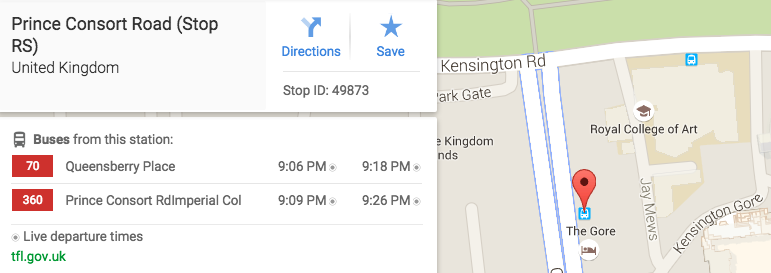
\includegraphics[width=1\textwidth]{figures/google_maps_tfl_data.png}
\caption{\label{fig:google_maps_tfl_data} Google Maps Using TfL Bus Arrival Data}
\end{figure}

Over 5,000 developers have registered for the open data \cite{open_data}, and around 200 travel apps are powered by it \cite{tfl_annual_report_13/14}. The most popular travel applications include \acrshort{tfl} Journey Planner, Google Maps (Figure \ref{fig:google_maps_tfl_data}), and Citymapper London. Given the departing location, destination, as well as departure time, these applications can provide suggested routes and travel times. Users can further customise their desired journey by specifying the desired walking distance, and accessibility requirements. Moreover, the \acrshort{tfl} Journey Planner and homepage status board were redesigned and integrated to provide customers planning their trip with a textual warning message if their route is likely to be affected by upgrade work or other disruptions \cite{tfl_annual_report_13/14}.

\par However, there are currently no applications that give predictions on travel times and warnings on potential delays. The estimated travel time shown in apps is extracted from the \acrshort{tfl} Journey Planner Bus Timetables. This information does not capture the real time delays according to instant traffic conditions.
